%package list
\documentclass{article}
\usepackage[top=3cm, bottom=3cm, outer=3cm, inner=3cm]{geometry}
\usepackage{multicol}
\usepackage{graphicx}
\usepackage{url}
%\usepackage{cite}
\usepackage{hyperref}
\usepackage{array}
%\usepackage{multicol}
\newcolumntype{x}[1]{>{\centering\arraybackslash\hspace{0pt}}p{#1}}
\usepackage{natbib}
\usepackage{pdfpages}
\usepackage{multirow}
\usepackage[normalem]{ulem}
\useunder{\uline}{\ul}{}
\usepackage{svg}
\usepackage{xcolor}
\usepackage{listings}
\lstdefinestyle{ascii-tree}{
    literate={├}{|}1 {─}{--}1 {└}{+}1 
  }
\lstset{basicstyle=\ttfamily,
  showstringspaces=false,
  commentstyle=\color{red},
  keywordstyle=\color{blue}
}
%\usepackage{booktabs}
\usepackage{caption}
\usepackage{subcaption}
\usepackage{float}
\usepackage{array}

\newcolumntype{M}[1]{>{\centering\arraybackslash}m{#1}}
\newcolumntype{N}{@{}m{0pt}@{}}


%%%%%%%%%%%%%%%%%%%%%%%%%%%%%%%%%%%%%%%%%%%%%%%%%%%%%%%%%%%%%%%%%%%%%%%%%%%%
%%%%%%%%%%%%%%%%%%%%%%%%%%%%%%%%%%%%%%%%%%%%%%%%%%%%%%%%%%%%%%%%%%%%%%%%%%%%
\newcommand{\itemEmail}{- Wiliam Herderson Choquehuanca Berna}
\newcommand{\itemStudent}{ - Ajra Huacso Jeans Anthony}
\newcommand{\itemCourse}{Programación Web 2}
\newcommand{\itemCourseCode}{20232208}
\newcommand{\itemSemester}{I}
\newcommand{\itemUniversity}{Universidad Nacional de San Agustín de Arequipa}
\newcommand{\itemFaculty}{Facultad de Ingeniería de Producción y Servicios}
\newcommand{\itemDepartment}{Departamento Académico de Ingeniería de Sistemas e Informática}
\newcommand{\itemSchool}{Escuela Profesional de Ingeniería de Sistemas}
\newcommand{\itemAcademic}{2024 - A}
\newcommand{\itemInput}{Del 28 Abril 2024}
\newcommand{\itemOutput}{Al 3 Mayo 2024}
\newcommand{\itemPracticeNumber}{01}
\newcommand{\itemTheme}{DOCKER}
%%%%%%%%%%%%%%%%%%%%%%%%%%%%%%%%%%%%%%%%%%%%%%%%%%%%%%%%%%%%%%%%%%%%%%%%%%%%
%%%%%%%%%%%%%%%%%%%%%%%%%%%%%%%%%%%%%%%%%%%%%%%%%%%%%%%%%%%%%%%%%%%%%%%%%%%%

\usepackage[english,spanish]{babel}
\usepackage[utf8]{inputenc}
\AtBeginDocument{\selectlanguage{spanish}}
\renewcommand{\figurename}{Figura}
\renewcommand{\refname}{Referencias}
\renewcommand{\tablename}{Tabla} %esto no funciona cuando se usa babel
\AtBeginDocument{%
	\renewcommand\tablename{Tabla}
}

\usepackage{fancyhdr}
\pagestyle{fancy}
\fancyhf{}
\setlength{\headheight}{30pt}
\renewcommand{\headrulewidth}{1pt}
\renewcommand{\footrulewidth}{1pt}
\fancyhead[L]{\raisebox{-0.2\height}{
\includegraphics[width=3cm]{img/logo_episunsa.png}}}
\fancyhead[C]{\fontsize{7}{7}\selectfont	\itemUniversity \\ \itemFaculty \\ \itemDepartment \\ \itemSchool \\ \textbf{\itemCourse}}
\fancyhead[R]{\raisebox{-0.2\height}{
\includegraphics[width=1.2cm]{img/logo_abet}}}
\fancyfoot[L]{Estudiante Juan Perez Perez}
\fancyfoot[C]{\itemCourse}
\fancyfoot[R]{Página \thepage}

% para el codigo fuente
\usepackage{listings}
\usepackage{color, colortbl}
\definecolor{dkgreen}{rgb}{0,0.6,0}
\definecolor{gray}{rgb}{0.5,0.5,0.5}
\definecolor{mauve}{rgb}{0.58,0,0.82}
\definecolor{codebackground}{rgb}{0.95, 0.95, 0.92}
\definecolor{tablebackground}{rgb}{0.8, 0, 0}

\lstset{frame=tb,
	language=bash,
	aboveskip=3mm,
	belowskip=3mm,
	showstringspaces=false,
	columns=flexible,
	basicstyle={\small\ttfamily},
	numbers=none,
	numberstyle=\tiny\color{gray},
	keywordstyle=\color{blue},
	commentstyle=\color{dkgreen},
	stringstyle=\color{mauve},
	breaklines=true,
	breakatwhitespace=true,
	tabsize=3,
	backgroundcolor= \color{codebackground},
}

\begin{document}
	
	\vspace*{10px}
	
	\begin{center}	
		\fontsize{17}{17} \textbf{ Informe de Laboratorio \itemPracticeNumber}
	\end{center}
	\centerline{\textbf{\Large Tema: \itemTheme}}
	%\vspace*{0.5cm}	

	\begin{flushright}
		\begin{tabular}{|M{2.5cm}|N|}
			\hline 
			\rowcolor{tablebackground}
			\color{white} \textbf{Nota}  \\
			\hline 
			     \\[30pt]
			\hline 			
		\end{tabular}
	\end{flushright}	

	\begin{table}[H]
		\begin{tabular}{|x{4.7cm}|x{4.8cm}|x{4.8cm}|}
			\hline 
			\rowcolor{tablebackground}
			\color{white} \textbf{Estudiante} & \color{white}\textbf{Escuela}  & \color{white}\textbf{Asignatura}   \\
			\hline 
			{\itemStudent \par \itemEmail} & \itemSchool & {\itemCourse \par Semestre: \itemSemester \par Código: \itemCourseCode}     \\
			\hline 			
		\end{tabular}
	\end{table}		
	
	\begin{table}[H]
		\begin{tabular}{|x{4.7cm}|x{4.8cm}|x{4.8cm}|}
			\hline 
			\rowcolor{tablebackground}
			\color{white}\textbf{Laboratorio} & \color{white}\textbf{Tema}  & \color{white}\textbf{Duración}   \\
			\hline 
			\itemPracticeNumber & \itemTheme & 04 horas   \\
			\hline 
		\end{tabular}
	\end{table}
	
	\begin{table}[H]
		\begin{tabular}{|x{4.7cm}|x{4.8cm}|x{4.8cm}|}
			\hline 
			\rowcolor{tablebackground}
			\color{white}\textbf{Semestre académico} & \color{white}\textbf{Fecha de inicio}  & \color{white}\textbf{Fecha de entrega}   \\
			\hline 
			\itemAcademic & \itemInput &  \itemOutput  \\
			\hline 
		\end{tabular}
	\end{table}

\item - AJRA HUACSO JEANS ANTHONY




\section{Ejercicio 1}
\textbf{Escriba una función que reciba el número de día de la fecha actual \texttt{new Date()} y devuelva el texto del día de la semana correspondiente. Por ejemplo, si recibe 0, devolvería “Domingo”.}

\begin{figure}[htbp]
    \centering
    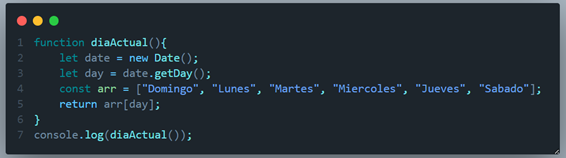
\includegraphics[width=0.4\linewidth]{1.png}
    \caption{Descripción de la captura 1 del ejercicio 1.}
\end{figure}

\section{Ejercicio 2}
\textbf{Escriba una página web que reciba un texto y al presionar un botón muestre el mismo texto invertido en otra sección (div). Por ejemplo, si se escribe “Hola”, se mostraría como “aloH”.}

\begin{figure}[htbp]
    \centering
    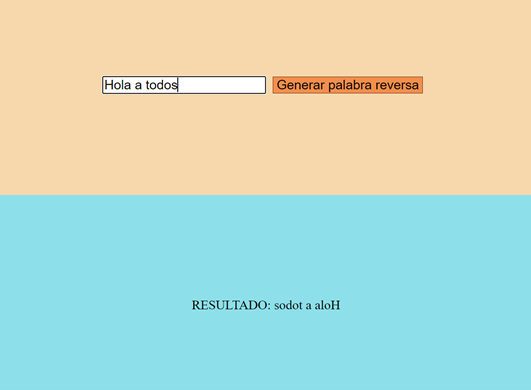
\includegraphics[width=0.4\linewidth]{3.png}
    \caption{Descripción de la captura 1 del ejercicio 2.}
\end{figure}
\begin{figure}[htbp]
    \centering
    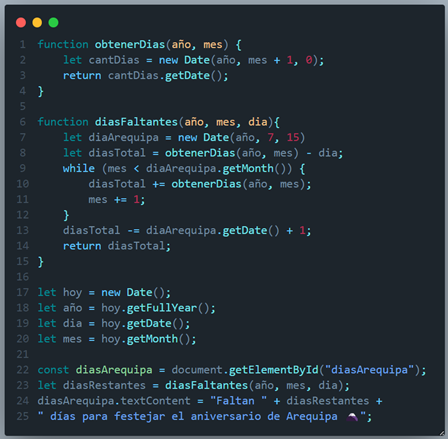
\includegraphics[width=0.4\linewidth]{4.png}
    \caption{Descripción de la captura 2 del ejercicio 2.}
\end{figure}

\section{Ejercicio 3}
\textbf{Escribir una página que muestre cuántos días faltan para el día de Arequipa!}

\begin{figure}[htbp]
    \centering
    
\includegraphics[width=0.4\linewidth]{5.png}
    \caption{Descripción de la captura 1 del ejercicio 3.}
\end{figure}
\begin{figure}[htbp]
    \centering
    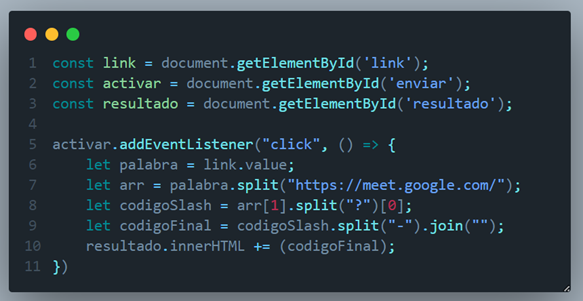
\includegraphics[width=0.4\linewidth]{6.png}
    \caption{Descripción de la captura 2 del ejercicio 3.}
\end{figure}

\section{Ejercicio 4}
\textbf{Escribir una página que reciba el URL de la sesión de Google Meet de hoy y devuelva el código de la sesión sin guiones separadores.}

\begin{figure}[htbp]
    \centering
    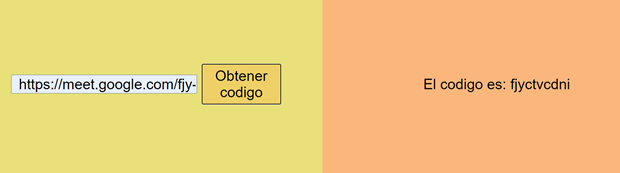
\includegraphics[width=0.4\linewidth]{7.png}
    \caption{Descripción de la captura 1 del ejercicio 4.}
\end{figure}
\begin{figure}[htbp]
    \centering
    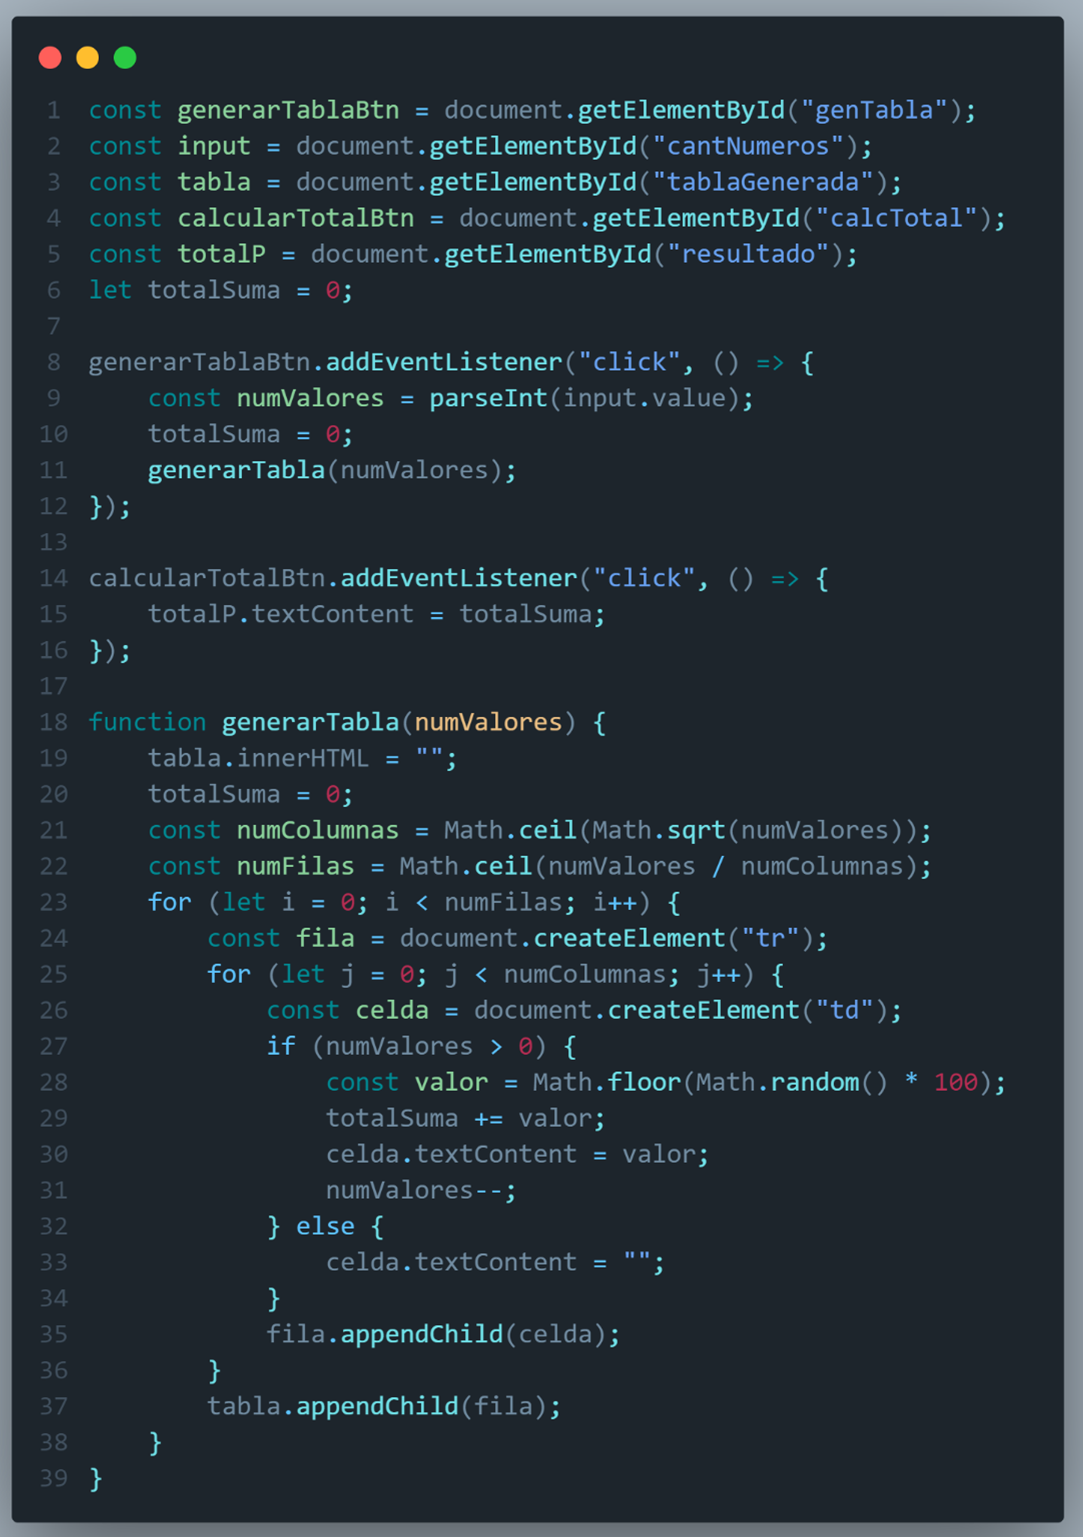
\includegraphics[width=0.4\linewidth]{8.png}
    \caption{Descripción de la captura 2 del ejercicio 4.}
\end{figure}

\section{Ejercicio 5}
\textbf{Escribir una página que permita calcular la suma de todos los valores de una tabla de valores dinámica. La idea es crear una página web con un formulario que te permita decir cuántos valores tendrá la tabla, luego, al enviar el formulario la tabla se debe crear dinámica y aleatoriamente, junto con otro botón de envío para calcular la suma.}

\begin{figure}[htbp]
    \centering
    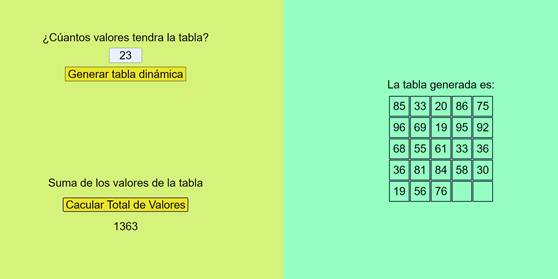
\includegraphics[width=0.4\linewidth]{9.png}
    \caption{Descripción de la captura 1 del ejercicio 5.}
\end{figure}
\begin{figure}[htbp]
    \centering
    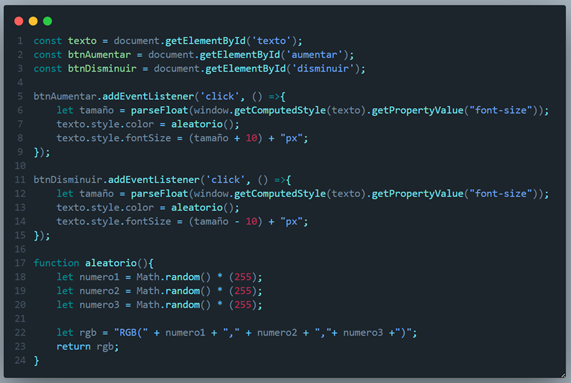
\includegraphics[width=0.4\linewidth]{10.png}
    \caption{Descripción de la captura 2 del ejercicio 5.}
\end{figure}

\section{Ejercicio 6}
\textbf{En su tarea deberán implementar las siguientes páginas.}
\subsection{Pagina1.html}
\textbf{Cree una página web con un texto y dos botones (al estilo del ejemplo del foco que se enciende y apaga) que permitan cambiar el tamaño de la letra de un texto, intente hacerlo también con los colores.}

\begin{figure}[htbp]
    \centering
    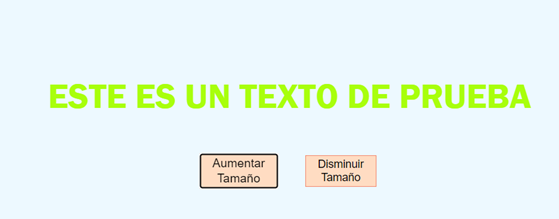
\includegraphics[width=0.4\linewidth]{11.png}
    \caption{Descripción de la captura 1 de la subsección Pagina1.html del ejercicio 6.}
\end{figure}
\begin{figure}[htbp]
    \centering
    
\includegraphics[width=0.4\linewidth]{12.png}
    \caption{Descripción de la captura 2 de la subsección Pagina1.html del ejercicio 6.}
\end{figure}
\begin{figure}[htbp]
    \centering
    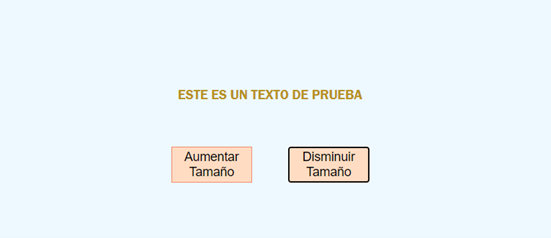
\includegraphics[width=0.4\linewidth]{13.png}
    \caption{Descripción de la captura 2 de la subsección Pagina1.html del ejercicio 6.}
\end{figure}

\subsection{Pagina2.html}
\textbf{Cree una página web que permita realizar las operaciones aritméticas, lógicas y de bits básicas, de manera dinámica (se podrá elegir cualquier operador) y se trabajará con dos argumentos.}

\begin{figure}[htbp]
    \centering
    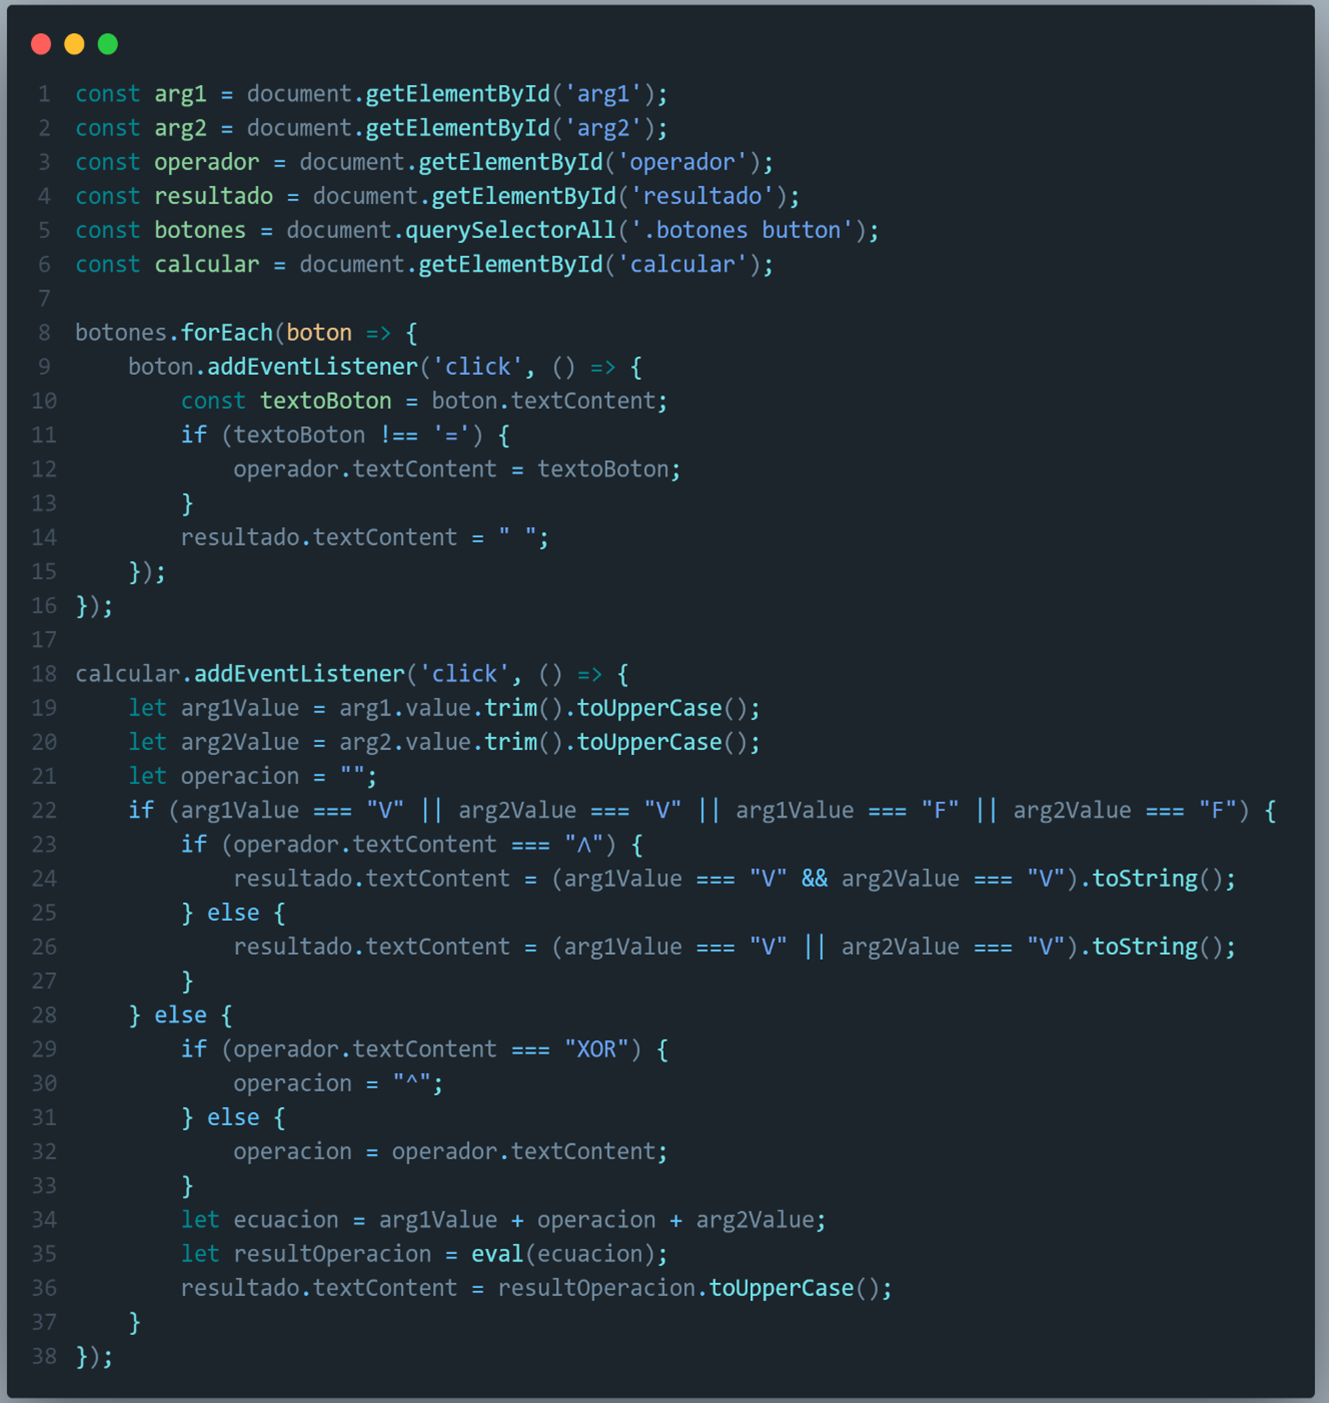
\includegraphics[width=0.4\linewidth]{14.png}
    \caption{Descripción de la captura 1 de la subsección Pagina2.html del ejercicio 6.}
\end{figure}
\begin{figure}[htbp]
    \centering
    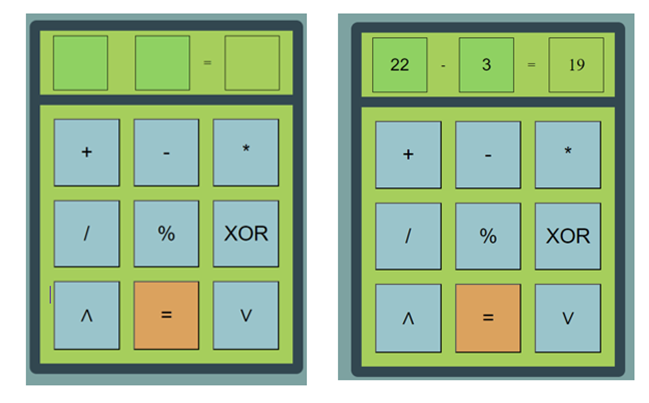
\includegraphics[width=0.4\linewidth]{15.png}
    \caption{Descripción de la captura 2 de la subsección Pagina2.html del ejercicio 6.}
\end{figure}

\section{Ejercicio 7}
\textbf{Resolver los 67 ejercicios de JavaScript en w3schools.com y subir un pantallazo con su nombre y apellido.}

\begin{figure}[htbp]
    \centering
    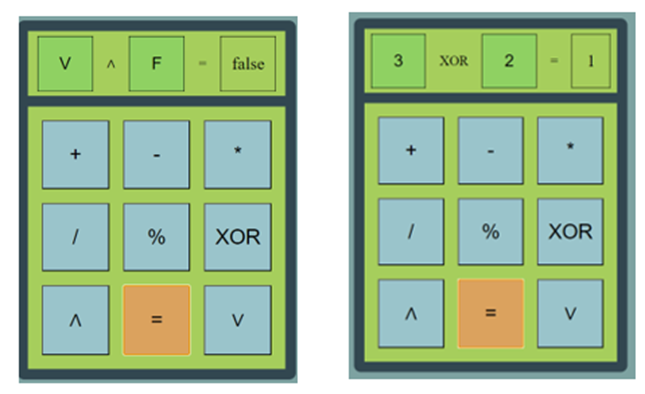
\includegraphics[width=0.4\linewidth]{16.png}
    \caption{Descripción de la captura 1 del ejercicio 7.}
\end{figure}
\begin{figure}[htbp]
    \centering
    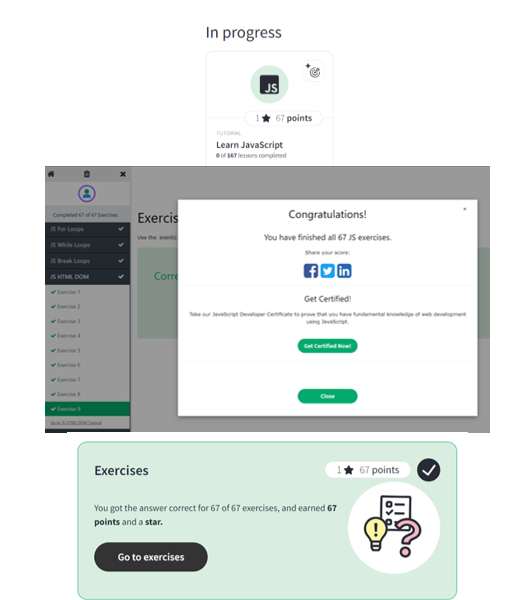
\includegraphics[width=0.4\linewidth]{17.png}
    \caption{Descripción de la captura 2 del ejercicio 7.}
\end{figure}
\item \textbf{URL de video de explicación:} \url{https://flip.com/72d8a713}
\item \textbf{URL de repositorio de GitHub:} \url{https://github.com/nuevo637/Lab2-Ejercicios_javascript}
        
\section{Referencias}
\begin{itemize}			
	\item \url{hhttps://www.w3schools.com/}
\end{itemize}	
	
%\clearpage
%\bibliographystyle{apalike}
%\bibliographystyle{IEEEtranN}
%\bibliography{bibliography}
			
\end{document}